\documentclass[12pt, a4paper]{article}
\usepackage[utf8]{inputenc}
\usepackage[T2A]{fontenc}
\usepackage{indentfirst, setspace}
\usepackage{tabularx, multirow}
\usepackage[normalem]{ulem}
\usepackage[style=russian]{csquotes}
\usepackage[english,russian]{babel}
\usepackage{hyperref}
\usepackage{ragged2e}
\usepackage{caption}
\usepackage{wrapfig}
\usepackage{amsmath}
\usepackage{tikz}
\makeatletter
\def\@biblabel#1{#1. }
\makeatother
\captionsetup{labelsep=endash}
\usepackage{listings}
\linespread{1.3}
\lstset{
  language=C++,
  basicstyle=\ttfamily\small,
  keywordstyle=\color{blue},
  breaklines=true,
  commentstyle=\color{green},
  stringstyle=\color{red},
  extendedchars=\true,
  showstringspaces=false,
  keepspaces=true,
}

\usepackage[left=2cm,right=2cm,
    top=2cm,bottom=2cm,bindingoffset=0cm]{geometry}\begin{document}
\begin{titlepage}
     \fontsize{12}{12}\selectfont

  {\centering

   \begin{bf}

    \begin{wrapfigure}{l}{10mm}
        
\includegraphics[width=17mm]{photo_2023-12-19.jpeg}
    \end{wrapfigure}


    \noindent Министерство науки и высшего образования Российской Федерации

    \noindent Федеральное государственное бюджетное образовательное учреждение высшего образования

    \noindent \enquote{Московский государственный технический университет

     \noindent имени Н.Э. Баумана

     \noindent (национальный исследовательский университет)}

    \noindent (МГТУ им. Н.Э. Баумана)

   \end{bf}
  }

  \vspace{0.4cm}

  {\setstretch{0.1}
   \noindent\rule{\textwidth}{1mm}
   \noindent\rule{\textwidth}{0.5mm}

  }

  \fontsize{14}{21}\selectfont

  \noindent\begin{tabularx}{\textwidth}{l >{\centering\arraybackslash}X}
   ФАКУЛЬТЕТ & \flqq Фундаментальные Науки\frqq \\ \cline{2-2}

   КАФЕДРА & ФН-12 \flqq Математическое моделирование\frqq \\ \cline{2-2}
  \end{tabularx}

  \vspace{1cm}


  \begin{center}
   \begin{bf}

    \fontsize{24}{36}\selectfont
    ОТЧЕТ

    \fontsize{20}{30}\selectfont
    ПО ЛАБОРАТОРНОЙ РАБОТЕ НА ТЕМУ:

    Длинная арифметика

   \end{bf}
  \end{center}

  \fontsize{14}{21}\selectfont
  \vspace{5cm}


  \noindent\begin{tabularx}{\textwidth}{ X >{\centering}p{4cm} p{1cm} c }
   Студент: & & & Мациевский И. М. \\ \cline{2-2} \cline{4-4}
   & \fontsize{10}{15}\selectfont дата, подпись & & \fontsize{10}{15}\selectfont Ф.И.О. \\
   Преподаватель: & & & Волкова Л. Л.\\ \cline{2-2} \cline{4-4}
   & \fontsize{10}{15}\selectfont дата, подпись & & \fontsize{10}{15}\selectfont Ф.И.О.
   \end{tabularx}

  \vspace{\fill}

  \begin{center}
   \it{Москва}, 2023
  \end{center}

  \thispagestyle{empty}
\end{titlepage}\newpage
\tableofcontents
\newpage
\section*{Введение}
\addcontentsline{toc}{section}{Введение}
\justifying
\textbf{Цель лабораторной работы}: составить 
структуру данных для хранения целых чисел с 
повышением ёмкости хранения по сравнению с базовым 
типом данных.

Для достижения поставленной цели требуется решить следующие 
\textbf{задачи}.
\begin{enumerate}
\item Реализовать 6 операторов сравнения.
\item Реализовать оператор присваивания.
\item Реализовать операторы сложения и вычитания 
двух структур длинных чисел в четверичной системе 
счисления.
\item Реализовать оператор четверичного сдвига 
вправо и влево.
\item Реализовать оператор остатка от деления 
структуры длинных чисел.
\end{enumerate}
\newpage
\section{Аналитическая часть}
\textbf{Длинная арифметика ---} это методика работы 
с числами, превышающими максимальные значения, 
предоставляемые базовыми типами данных языка 
программирования. Часто используется в задачах, 
требующих работы с очень большими числами, такие
задачи часто встречаются, например, в науке. 

Для хранения длинных чисел в лабораторной работе 
реализован класс $QuaternaryNumber$, объектом класса 
является массив цифр от 0 до 3 и дополнительный флаг
$isNegative$, принимающий значение $true$ в случае, 
когда число положительно и значение $false$, когда
число отрицательно.

Для работы с объектами класса перегружены операторы
сложения, вычитания, остатка от деления, 6 
операторов сравнения, оператор присваивания, реализованы операторы 
четверичного сдвига вправо и влево.
\newpage
\section{Конструкторская часть}
\textbf{Операторы сравнения}
\begin{enumerate}
	\item Оператор '==' сначала сравнивает знаки двух чисел, если знаки 
	одинаковы, то сравнивает два числа поразрядно, возвращает $true$ в 
	случае равенства чисел, иначе $false$.
	\item Оператор '!=' сравнивает два числа сначала по их знакам 
	и если знаки различны, сравнивает числа поразрядно, возвращает 
	$false$ в случае равенства чисел, иначе $true$.
	\item Оператор '<' сначала сравнивает знаки двух чисел, если знаки 
	одинаковы, то сравнивает два числа поразрядно, возвращает $false$, 
	если первое (по левую сторону от оператора) число больше второго или 
	равно ему, иначе $true$.
	\item Оператор '>' сначала сравнивает знаки двух чисел, если знаки 
	одинаковы, то сравнивает два числа поразрядно, возвращает $true$, 
	если первое (по левую сторону от оператора) число больше второго, 
	иначе $false$.
	\item Оператор '<=' сначала сравнивает знаки двух чисел, если знаки 
	одинаковы, то сравнивает два числа поразрядно, возвращает $false$, 
	если первое (по левую сторону от оператора) число больше второго, 
	иначе $true$.
	\item Оператор '>=' сначала сравнивает знаки двух чисел, если знаки 
	одинаковы, то сравнивает два числа поразрядно, возвращает $true$, 
	если первое (по левую сторону от оператора) число больше второго или 
	равно ему, иначе $false$.
	\item Оператор '< <=' сравнивает поразрядно модули двух чисел, 
	возвращает $true$, если первое (по левую сторону от оператора) число 
	по модулю меньше второго, иначе $false$.
	\item Оператор '> >=' сравнивает поразрядно модули двух чисел, 
	возвращает $true$, если первое (по левую сторону от оператора) число 
	по модулю больше второго, иначе $false$.
\end{enumerate}
\textbf{Остальные операторы}
\begin{enumerate}
	\item Оператор '> >' сдвигает цифры числа вправо на заданное 
	количество разрядов, освободившиеся разряды заполняет нулями.
	\item Оператор '< <' сдвигает цифры числа влево на заданное 
	количество разрядов, освободившиеся разряды заполняет нулями.
	\item Операторы '+' и '-' определяется знак суммы/разности в 
	зависимости от знаков операндов, после этого поразрядно 
	складываются/вычитаются модули двух чисел, используется 
	дополнительная переменная для операции "заема" из старшего 
	разряда и "добавления" в старший разряд.
	\item Оператор '\%' использует операцию вычитания для нахождения 
	остатка от деления.
	\item Оператор '=' копирует значения цифр и флага знака из одного 
	объекта в другой.
\end{enumerate}
\textbf{Вспомогательные функции и методы}
\begin{enumerate}
	\item $isEqual$ сначала сравнивает знаки двух чисел, если знаки 
	одинаковы, то сравнивает два числа поразрядно, возвращает $true$ в 
	случае равенства чисел, иначе $false$.
	\item $isEqual\_abs$ сравнивает модули двух чисел поразрядно, 
	возвращает $true$ в случае равенства чисел по модулю, иначе $false$.
	\item $isGreaterThan\_abs$ сравнивает модули двух чисел поразрядно, 
	возвращает $true$, если первое число по модулю больше второго, иначе 
	$false$.
	\item $isGreaterThan$ сначала сравнивает знаки двух чисел, если 
	знаки одинаковы, сравнивает модули двух чисел поразрядно, 
	возвращает $true$, если первое число больше второго, иначе $false$.
	\item $isLessThan\_abs$ сравнивает модули двух чисел поразрядно, 
	возвращает $true$, если первое число по модулю меньше второго, иначе 
	$false$.
	\item $isLessThan$ сначала сравнивает знаки двух чисел, если 
	знаки одинаковы, сравнивает модули двух чисел поразрядно, 
	возвращает $true$, если первое число меньше второго, иначе $false$.
	\item $print()$ выводит число на экран, учитывая его знак и 
	форматирование.
\end{enumerate}
\newpage
\section{Технологическая часть}
Для реализации выбран язык C++.
На листинге 1 представлена реализация программы
(Реализация~\ref{lst:label1})
\begin{lstlisting}[caption={Исходный код}, label={lst:label1}]
#include <iostream>
#include <cmath>
#include <iomanip>
using namespace std;

const int MAX_DIGITS = 10;

class QuaternaryNumber {
private:
    int digits[MAX_DIGITS];
    bool isNegative;

public:
    QuaternaryNumber() {
        for (int i = 0; i < MAX_DIGITS; ++i) {
            digits[i] = 0;
        }
        isNegative = false;
    }

    QuaternaryNumber(int value) {
        isNegative = value < 0;
        value = abs(value);

        for (int i = 0; i < MAX_DIGITS; ++i) {
            digits[i] = value % 4;
            value /= 4;
        }
    }

    // Операторы сравнения по модулю
    bool operator==(const QuaternaryNumber& other) const {
        return isEqual(other);
    }

    bool operator!=(const QuaternaryNumber& other) const {
        return !isEqual(other);
    }

    bool operator<<=(const QuaternaryNumber& other) const {
        return isLessThan_abs(other); //сравнение по модулю
    }

    bool operator>>=(const QuaternaryNumber& other) const {
        return isGreaterThan_abs(other); //сравнение по модулю
    }
    
    bool operator<(const QuaternaryNumber& other) const {
        return isLessThan(other);
    }

    bool operator>(const QuaternaryNumber& other) const {
        return isGreaterThan(other);
    }

    bool operator<=(const QuaternaryNumber& other) const {
        return !isGreaterThan(other);
    }

    bool operator>=(const QuaternaryNumber& other) const {
        return !isLessThan(other);
    }

    // Оператор присваивания
    QuaternaryNumber& operator=(const QuaternaryNumber& other) {
        if (this != &other) {
            for (int i = 0; i < MAX_DIGITS; ++i) {
                digits[i] = other.digits[i];
            }
            isNegative = other.isNegative;
        }
        return *this;
    }

    // Операции сложения и вычитания
   QuaternaryNumber operator+(const QuaternaryNumber& other) const {
    QuaternaryNumber result;
    int carry = 0;

    // Определяем знак результата
    if (isNegative && !other.isNegative) {
        if (*this >>= other) {
            result.isNegative = true;
        } else {
            result.isNegative = false;
        }
    } else if (!isNegative && other.isNegative) {
        if (*this >>= other) {
            result.isNegative = false;
        } else {
            result.isNegative = true;
        }
    } else if (isNegative && other.isNegative) {
        result.isNegative = true;
    } else {
        result.isNegative = false;
    }
    bool isZero = true;
    // Складываем числа по модулю
    for (int i = 0; i < MAX_DIGITS; ++i) {
        int sum;

        if (isNegative && !other.isNegative) {
            if (*this >>= other) {
                sum = digits[i] - other.digits[i] - carry;
            }
            else {
            sum = other.digits[i] - digits[i] - carry;
            }
        }
        else if (!isNegative && other.isNegative) {
            if (*this >>= other) {
                sum = digits[i] - other.digits[i] - carry;
            }
            else {
            sum = other.digits[i] - digits[i] - carry;
            }
        }
        else if (isNegative && other.isNegative) {
            sum = other.digits[i] + digits[i] + carry;
        }
        else {
            sum = digits[i] + other.digits[i] + carry;
        }

        if (sum < 0) {
            sum += 4;
            carry = 1;
        }
        else if (sum > 3) {
            carry = 1;
        }
        else {
            carry = 0;
        }
        if (sum % 4 != 0) {
            isZero = false;
        }
        result.digits[i] = sum % 4;
    }
    if (carry > 0) {
        for (int i = MAX_DIGITS - 1; i >= 0; --i) {
            if (result.digits[i] != 0) {
                result.digits[i - 1] += carry;
                carry = 0;
                break;
            }
        }
    }
    if (isZero) {
        result.isNegative = false;
    }
    return result;
}


    QuaternaryNumber operator-(const QuaternaryNumber& other) const {
     QuaternaryNumber result;
     int carry = 0;

     // Определяем знак результата
     if (isNegative && other.isNegative) {
         if (*this >>= other) {
             result.isNegative = true;
         } else {
             result.isNegative = false;
         }
     } else if (!isNegative && !other.isNegative) {
         if (*this >>= other) {
             result.isNegative = false;
         } else {
             result.isNegative = true;
         }
     } else if (isNegative && !other.isNegative) {
         result.isNegative = true;
     } else {
         result.isNegative = false;
     }
     bool isZero = true;
     // Складываем числа по модулю
     for (int i = 0; i < MAX_DIGITS; ++i) {
         int sum;

         if (isNegative && other.isNegative) {
             if (*this >>= other) {
                 sum = digits[i] - other.digits[i] - carry;
             }
             else {
             sum = other.digits[i] - digits[i] - carry;
             }
         }
         else if (!isNegative && !other.isNegative) {
             if (*this >>= other) {
                 sum = digits[i] - other.digits[i] - carry;
             }
             else {
             sum = other.digits[i] - digits[i] - carry;
             }
         }
         else if (isNegative && !other.isNegative) {
             sum = other.digits[i] + digits[i] + carry;
         }
         else {
             sum = digits[i] + other.digits[i] + carry;
         }

         if (sum < 0) {
             sum += 4;
             carry = 1;
         }
         else if (sum > 3) {
             carry = 1;
         }
         else {
             carry = 0;
         }
         if (sum % 4 != 0) {
             isZero = false;
         }
         result.digits[i] = sum % 4;
     }
     if (carry > 0) {
         for (int i = MAX_DIGITS - 1; i >= 0; --i) {
             if (result.digits[i] != 0) {
                 result.digits[i - 1] += carry;
                 carry = 0;
                 break;
             }
         }
     }
    if (isZero) {
        result.isNegative = false;
    }
     return result;
 }


    // Другие операции
    QuaternaryNumber operator<<(int shift) const {
        QuaternaryNumber result = *this;
        for (int i = 0; i < shift; ++i) {
            for (int j = MAX_DIGITS - 1; j > 0; --j) {
                result.digits[j] = result.digits[j - 1];
            }
            result.digits[0] = 0;
        }
        return result;
    }

    QuaternaryNumber operator>>(int shift) const {
        QuaternaryNumber result = *this;
        for (int i = 0; i < shift; ++i) {
            for (int j = 0; j < MAX_DIGITS - 1; ++j) {
                result.digits[j] = result.digits[j + 1];
            }
            result.digits[MAX_DIGITS - 1] = 0;
        }
        return result;
    }

    QuaternaryNumber operator%(const QuaternaryNumber& divisor) const {
        QuaternaryNumber dividend = *this;
        if (dividend.isNegative == divisor.isNegative) {
            while (dividend >= divisor) {
                dividend = dividend - divisor;
            }
        }
        else if (dividend.isNegative) {
            while (dividend.isNegative) {
                dividend = dividend + divisor;
            }
        }
        else {
            while (!dividend.isNegative) {
                dividend = dividend + divisor;
            }
        }
        return dividend;
    }

    // Вспомогательные функции
    bool isEqual(const QuaternaryNumber& other) const {
        if (isNegative != other.isNegative) {
            return false;
        }
        for (int i = 0; i < MAX_DIGITS; ++i) {
            if (digits[i] != other.digits[i]) {
                return false;
            }
        }
        return true;
    }
    
    bool isEqual_abs(const QuaternaryNumber& other) const {
            for (int i = 0; i < MAX_DIGITS; ++i) {
                if (digits[i] != other.digits[i]) {
                    return false;
                }
            }
            return true;
        }

    bool isGreaterThan_abs(const QuaternaryNumber& other) const {
            for (int i = MAX_DIGITS - 1; i >= 0; --i) {
                if (digits[i] > other.digits[i]) {
                    return true;
                } else if (digits[i] < other.digits[i]) {
                    return false;
                }
            }
            return false;
        }
    
    bool isGreaterThan(const QuaternaryNumber& other) const {
        if (isNegative and !other.isNegative) {
            return false;
        }
        else if (!isNegative and other.isNegative) {
            return true;
        }
        else if (!isNegative and !other.isNegative) {
            for (int i = MAX_DIGITS - 1; i >= 0; --i) {
                if (digits[i] > other.digits[i]) {
                    return true;
                } else if (digits[i] < other.digits[i]) {
                    return false;
                }
            }
            return false;
        }
        else {
            for (int i = MAX_DIGITS - 1; i >= 0; --i) {
                if (digits[i] > other.digits[i]) {
                    return false;
                } else if (digits[i] < other.digits[i]) {
                    return true;
                }
            }
            return true;
        }
    }
    
    bool isLessThan_abs(const QuaternaryNumber& other) const {
        return !isEqual_abs(other) && !isGreaterThan_abs(other);
    }
    
    bool isLessThan(const QuaternaryNumber& other) const {
        return !isEqual(other) && !isGreaterThan(other);
    }

    // Вывод числа
    void print() const {
        if (isNegative) {
            cout << '-';
        }

        for (int i = MAX_DIGITS - 1; i >= 0; --i) {
            cout << digits[i];
        }

        cout << endl;
    }
};

int main() {
    int x, y;
    cout << "Введите первое число" << endl;
    cin >> x;
    cout << "Введите второе число" << endl;
    cin >> y;
    QuaternaryNumber a(x);
    QuaternaryNumber b(y);

    QuaternaryNumber sum = a + b;
    QuaternaryNumber diff = a - b;
    QuaternaryNumber leftShift = a << 2;
    QuaternaryNumber rightShift = a >> 1;
    QuaternaryNumber modulo = a % b;

    // Проверка операторов сравнения
    bool isEqual = (a == b);
    bool isNotEqual = (a != b);
    bool isLessThan = (a < b);
    bool isGreaterThan = (a > b);
    bool isLessOrEqual = (a <= b);
    bool isGreaterOrEqual = (a >= b);

    // Проверка оператора присваивания
    QuaternaryNumber assigned = a;

    cout << "a: ";
    a.print();

    cout << "b: ";
    b.print();

    cout << "a + b: ";
    sum.print();

    cout << "a - b: ";
    diff.print();

    cout << "a << 2: ";
    leftShift.print();

    cout << "a >> 1: ";
    rightShift.print();

    cout << "a % b: ";
    modulo.print();

    cout << "a == b: " << boolalpha << isEqual << endl;
    cout << "a != b: " << boolalpha << isNotEqual << endl;
    cout << "a < b: " << boolalpha << isLessThan << endl;
    cout << "a > b: " << boolalpha << isGreaterThan << endl;
    cout << "a <= b: " << boolalpha << isLessOrEqual << endl;
    cout << "a >= b: " << boolalpha << isGreaterOrEqual << endl;

    cout << "Assigned: ";
    assigned.print();

    return 0;
}
\end{lstlisting}
\newpage
\textbf{Примеры работы.}
На рисунках 1---8 представлены примеры работы программы для расчета выражений
в длинной арифметике.
\begin{enumerate}
	\item Входные файлы: два положительных числа:
	Результат приведён на рис.~\ref{img:grap1}.
	\begin{figure}[h]
  		\center{
\includegraphics[scale=0.7]{ex1.png}}
  		\caption{Пример работы 1}
  		\label{img:grap1}
	\end{figure}
	\item Входные файлы: первое число положительно, второе отрицательно.
	Результат приведён на рис.~\ref{img:grap2}.
	\begin{figure}[h]
  		\center{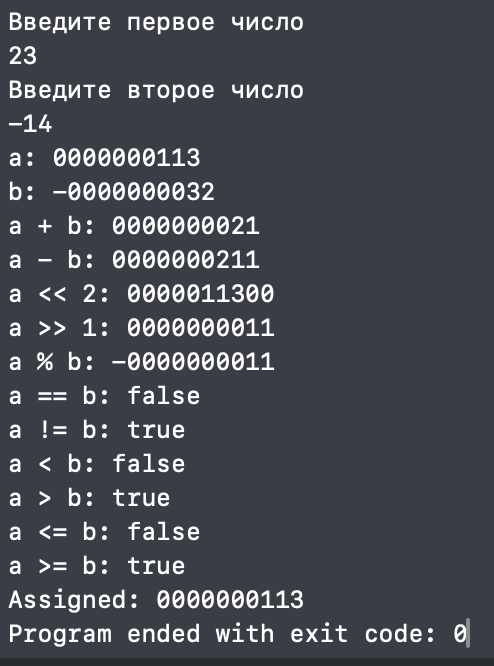
\includegraphics[scale=0.7]{ex2.png}}
  		\caption{Пример работы 2}
  		\label{img:grap2}
	\end{figure}
	\newpage
	\item Входные файлы: два отрицательных числа.
	Результат приведён на рис.~\ref{img:grap3}.
	\begin{figure}[h]
  		\center{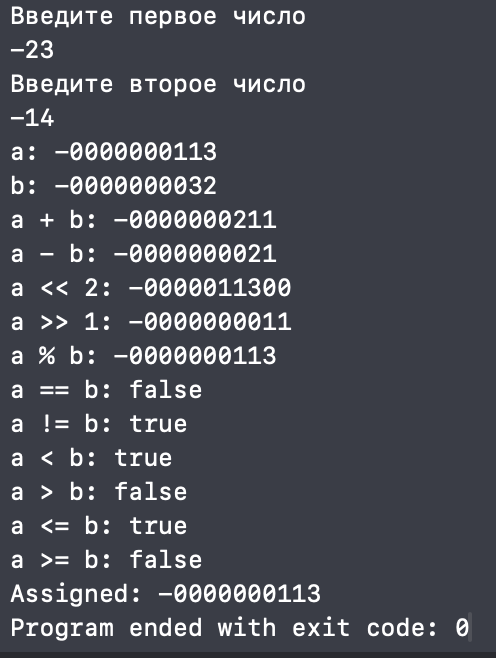
\includegraphics[scale=0.7]{ex3.png}}
  		\caption{Пример работы 3}
  		\label{img:grap3}
	\end{figure}
	\item Входные файлы: первое число отрицательно, второе положительно.
	Результат приведён на рис.~\ref{img:grap4}.
	\begin{figure}[h]
  		\center{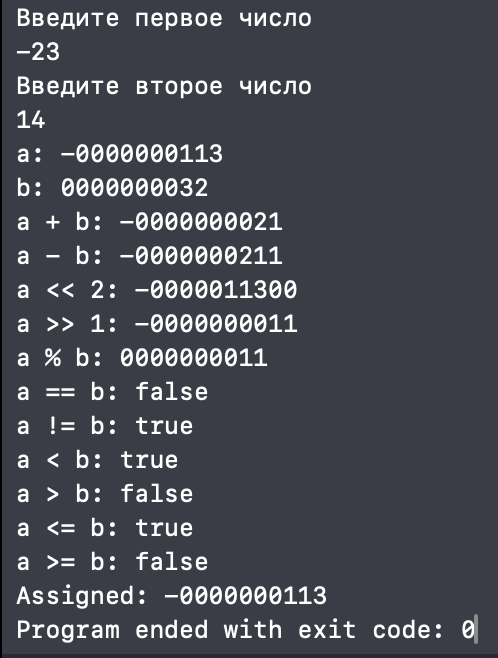
\includegraphics[scale=0.7]{ex4.png}}
  		\caption{Пример работы 4}
  		\label{img:grap4}
	\end{figure}
	\newpage
	\item Входные файлы: числа, равные по модулю и противоположные по 
	знаку.
	Результат приведён на рис.~\ref{img:grap5}.
	\begin{figure}[h]
  		\center{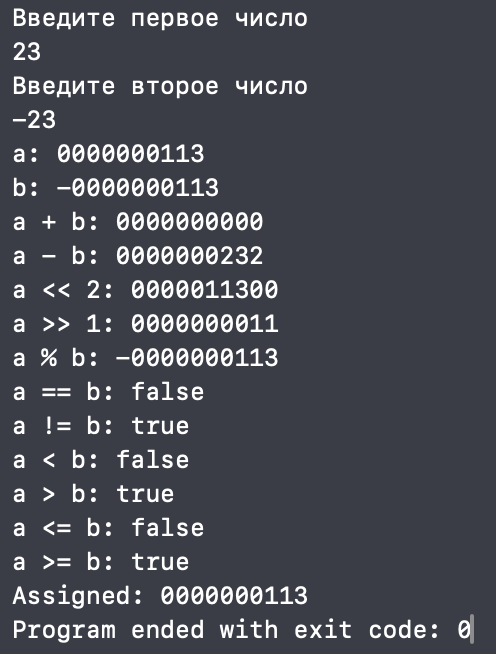
\includegraphics[scale=0.7]{ex5.png}}
  		\caption{Пример работы 5}
  		\label{img:grap5}
	\end{figure}
	\item Входные файлы: равные числа.
	Результат приведён на рис.~\ref{img:grap6}.
	\begin{figure}[h]
  		\center{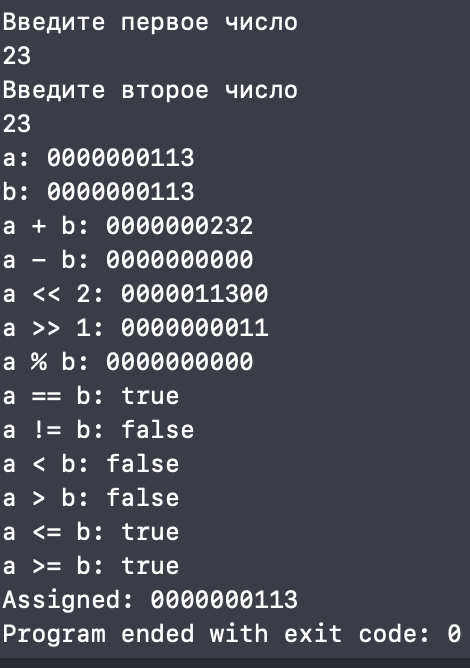
\includegraphics[scale=0.7]{ex6.png}}
  		\caption{Пример работы 6}
  		\label{img:grap6}
	\end{figure}
	\newpage
	\item Входные файлы: первое число нуль, второе число положительно.
	Результат приведён на рис.~\ref{img:grap7}.
	\begin{figure}[h]
  		\center{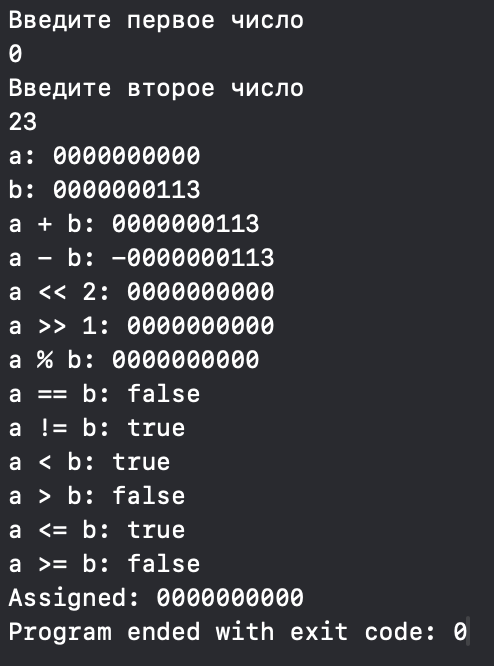
\includegraphics[scale=0.7]{ex7.png}}
  		\caption{Пример работы 7}
  		\label{img:grap7}
	\end{figure}
	\item Входные файлы: первое число нуль, второе число отрицательно:
	Результат приведён на рис.~\ref{img:grap8}.
	\begin{figure}[h]
  		\center{
\includegraphics[scale=0.7]{ex8.png}}
  		\caption{Пример работы 8}
  		\label{img:grap8}
	\end{figure}
\end{enumerate}
\newpage
\section*{Заключение}
\addcontentsline{toc}{section}{Заключение}
Цель достигнута: разработана структура данных для хранения целых чисел с 
хранением 10 разрядов. В результате выполнения лабораторной работы были 
выполнены все задачи.
\begin{enumerate}
\item Реализовано 6 операторов сравнения.
\item Реализован оператор присваивания.
\item Реализованы операторы сложения и вычитания 
двух структур длинных чисел в четверичной системе 
счисления.
\item Реализован оператор четверичного сдвига 
вправо и влево.
\item Реализован оператор остатка от деления 
структуры длинных чисел.
\end{enumerate}
\newpage
\begin{center}
\begin{thebibliography}{}
\addcontentsline{toc}{section}{Список используемых источников}
\bibitem{book}Неспирный В.Н., Длинная арифметика: научная статья 2010. – 
13 с.
\end{thebibliography}
\end{center}
\end{document}
